%!TEX encoding = UTF-8 Unicode
%!TEX root = ../lect-w10.tex

%%%


%\begin{Slide}{TODO: Begrepp att förklara}
%  Tänk igenom ordningen:
%  \begin{itemize}
%    \item OO, arv, supertyp, subtyp, bastyp, polymorfism, ...
%  \end{itemize}
%\end{Slide}


\Subsection{Vad är arv?}

\begin{Slide}{Vad är arv?}

\begin{minipage}{0.4\textwidth}
\raggedright Arv \Eng{inheritance} beskriver relationen \\
$X$ \Emph{är en} $Y$

\end{minipage}
\begin{minipage}{0.4\textwidth}
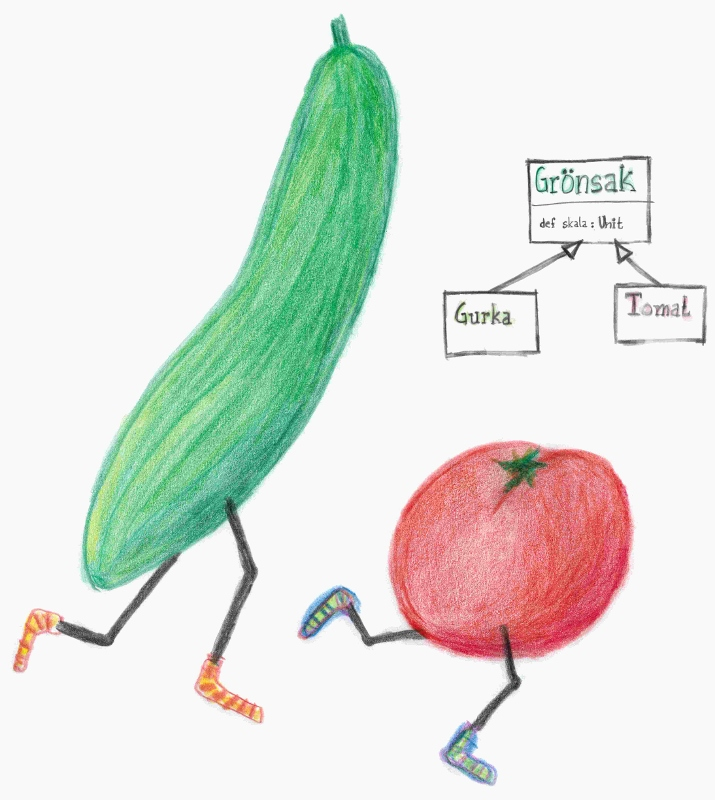
\includegraphics[width=1.5\textwidth]{../img/gurka-tomat-715x800}
\end{minipage}
\end{Slide}


\begin{Slide}{Varför behövs arv?}
\begin{itemize}
\item Man kan använda arv för att dela upp kod i:
\begin{itemize}
\item \Emph{generella} (gemensamma) delar och
\item \Emph{specifika} (specialanpassade) delar.
\end{itemize}

\item Man kan åstadkomma \Emph{kontrollerad flexibilitet}:
\begin{itemize}
\item Klientkod kan \Emph{utvidga} \Eng{extend} ett givet API med egna specifika tillägg.
\end{itemize}

\item Man kan använda arv för att deklarera en gemensam \Emph{bastyp} så att generiska samlingar kan ges en mer specifik elementtyp.
\begin{itemize}
\item Det räcker att man vet bastypen för att kunna anropa gemensamma metoder på alla element i samlingen.
\end{itemize}
\end{itemize}
\end{Slide}



\begin{Slide}{Klassdiagram med UML (Unified Modeling Language)}
\begin{center}
\begin{tikzpicture}
\node (Class) [umlclass, rectangle split parts = 3, xshift = -2cm, yshift=-1.5cm, text width = 4.2cm, scale=0.8]  {
            \textbf{\centerline{Name}}
            \nodepart[]{second}attr1: Type \newline attr2: Type
            \nodepart[]{third}method1(a: Type): Type \newline  method2(b: Type): Type
       };
\node (explain1)[above of = Class, yshift=1cm, text width=5.5cm]{En klass, i ett \Emph{UML}-diagram kan ha 3 delar:};
%\node (explain2)[below of = Class, yshift=-1cm]{Ibland utelämnar man attribut/metoder};

\pause

\node [umlclass, rectangle split parts = 3]  at (4,0) (Robot) {
            \textbf{\centerline{Robot}}
            \nodepart[]{second}name: String
            \nodepart[]{third}work(): Unit
       };
\node [umlclass, rectangle split parts = 3]  at (4, -3) (TalkingRobot)  {
            \textbf{\centerline{TalkingRobot}}
            \nodepart[]{second} phrase: String
            \nodepart[]{third}talk(): Unit
        };
\draw[umlarrow] (TalkingRobot.north) -- ++(0,0.8) -| (Robot.south);

\end{tikzpicture}
\end{center}
Mer om UML-diagram i pfk, OMD.\\
\href{https://en.wikipedia.org/wiki/Class_diagram}{\SlideFontTiny en.wikipedia.org/wiki/Class\_diagram}

\end{Slide}

\begin{Slide}{Exempel: Robot}
\begin{center}
\newcommand{\TextBox}[1]{\raisebox{0pt}[1em][0.5em]{#1}}
\begin{tikzpicture}[inner sep=0.5em]
\node [umlclass, rectangle split parts = 2, xshift=0cm, text width=4cm] (AbstractRobot)  {
           \textit{\textbf{\centerline{\TextBox{Robot}}}}
           \nodepart[]{second}\TextBox{\code{def work(): Unit}}
       };

\node [umlclass, rectangle split parts = 2, text width=4cm]  at (3cm,-3cm) (MuteRobot) {
           \textbf{\centerline{\TextBox{MuteRobot}}}
           \nodepart[]{second} \TextBox{~}
       };

\node [umlclass, rectangle split parts = 2, text width=4cm] at (-3cm,-3cm) (TalkingRobot)  {
           \textbf{\centerline{\TextBox{TalkingRobot}}}
           \nodepart[]{second} \TextBox{\code{def talk(): Unit}}
       };
\draw[umlarrow] (TalkingRobot.north) -- ++(0,0.5) -| (AbstractRobot.south);
\draw[umlarrow] (MuteRobot.north) -- ++(0,0.5) -| (AbstractRobot.south);
\end{tikzpicture}
\end{center}
Ibland utelämnar man attribut och/eller metoder för att minska på antalet detaljer och ge överblick.
\end{Slide}


\begin{Slide}{Behovet av gemensam bastyp}\SlideFontSmall
\begin{REPL}
scala> class Gurka(val vikt: Int)

scala> class Tomat(val vikt: Int)

scala> val gurkor = Vector(new Gurka(200), new Gurka(300))
gurkor: scala.collection.immutable.Vector[Gurka] =
  Vector(Gurka@60856961, Gurka@2fd953a6)

scala> gurkor.map(_.vikt)
res0: scala.collection.immutable.Vector[Int] = Vector(200, 300)

scala> val grönsaker = Vector(new Gurka(200), new Tomat(42))
grönsaker: scala.collection.immutable.Vector[Object] =
  Vector(Gurka@669253b7, Tomat@5305c37d)

scala> grönsaker.map(_.vikt)
<console>:15: error: value vikt is not a member of Object
       grönsaker.map(_.vikt)
\end{REPL}
Hur ordna en mer specifik typ än \code{Vector[Object]}? \pause$\rightarrow$ Skapa en \Emph{bastyp}!
\end{Slide}




\begin{Slide}{Skapa en gemensam bastyp}
Typen \textit{\textbf{\texttt{Grönsak}}} är en \Emph{bastyp} i nedan arvshierarki:

\vspace{1em}
\begin{center}
\newcommand{\TextBox}[1]{\raisebox{0pt}[1em][0.5em]{#1}}
\tikzstyle{umlclass}=[rectangle, draw=black,  thick, anchor=north, text width=2cm, rectangle split, rectangle split parts = 3]
\begin{tikzpicture}[inner sep=0.5em]
\node [umlclass, rectangle split parts = 1, xshift=0cm] (BaseType)  {
            \textit{\textbf{\centerline{\TextBox{\code{Grönsak}}}}}
            %\nodepart[]{second}\TextBox{\code{val vikt: Int}}
        };

\node [umlclass, rectangle split parts = 1]  at (2cm,-2cm) (SubType1) {
            \textbf{\centerline{\TextBox{\code{Gurka}}}}
            %\nodepart[]{second} \TextBox{~}
        };

\node [umlclass, rectangle split parts = 1] at (-2cm,-2cm) (SubType2)  {
            \textbf{\centerline{\TextBox{\code{Tomat}}}}
            %\nodepart[]{second} \TextBox{talk(): void}
        };
\draw[umlarrow] (SubType1.north) -- ++(0,0.5) -| (BaseType.south);
\draw[umlarrow] (SubType2.north) -- ++(0,0.5) -| (BaseType.south);
\end{tikzpicture}

\pause
\vspace{2em} Pilen ~ \tikz\draw[umlarrow] (0,0) -- (0,0.5); ~ betecknar \Emph{arv} och utläses ''\Alert{är en}''

\pause
{\vspace{1em}\SlideFontSmall 
Typerna \code{Tomat} och \code{Gurka} är \Emph{subtyper} till den \Emph{abstrakta} typen \code{Grönsak}.\\
En typ kallas abstrakt om den inte kan instansieras.
}
\end{center}
\end{Slide}







\begin{Slide}{Skapa en gemensam bastyp med \texttt{trait} och \texttt{extends}}\SlideFontSmall
Med \code{trait Grönsak} kan klasserna \code{Gurka} och \code{Tomat} få en gemensam \Emph{bastyp} genom att båda \Emph{subtyperna} gör \code{extends Grönsak}:
\begin{REPL}
scala> trait Grönsak

scala> class Gurka(val vikt: Int) extends Grönsak

scala> class Tomat(val vikt: Int) extends Grönsak

scala> val grönsaker = Vector(new Gurka(200), new Tomat(42))
grönsaker: scala.collection.immutable.Vector[Grönsak] =
  Vector(Gurka@3dc4ed6f, Tomat@2823b7c5)


\end{REPL}
\pause
Men det är fortfarande inte som vi vill ha det:
\begin{REPLnonum}
scala> grönsaker.map(_.vikt)
<console>:15: error: value vikt is not a member of Grönsak
       grönsaker.map(_.vikt)
\end{REPLnonum}
\end{Slide}



\begin{Slide}{En gemensam bastyp med gemensamma delar}\SlideFontSmall
Placera gemensamma medlemmar i bastypen:

\vspace{1em}
\begin{center}
\newcommand{\TextBox}[1]{\raisebox{0pt}[1em][0.5em]{#1}}
\tikzstyle{umlclass}=[rectangle, draw=black,  thick, anchor=north, text width=3cm, rectangle split, rectangle split parts = 3]
\begin{tikzpicture}[inner sep=0.5em]
\node [umlclass, rectangle split parts = 2, xshift=0cm] (BaseType)  {
            \textit{\textbf{\centerline{\TextBox{\code{Grönsak}}}}}
            \nodepart[]{second}\TextBox{\code{val vikt: Int}}
        };

\node [umlclass, rectangle split parts = 1]  at (2cm,-3cm) (SubType1) {
            \textbf{\centerline{\TextBox{\code{Gurka}}}}
            %\nodepart[]{second} \TextBox{~}
        };

\node [umlclass, rectangle split parts = 1] at (-2cm,-3cm) (SubType2)  {
            \textbf{\centerline{\TextBox{\code{Tomat}}}}
            %\nodepart[]{second} \TextBox{talk(): void}
        };
\draw[umlarrow] (SubType1.north) -- ++(0,0.5) -| (BaseType.south);
\draw[umlarrow] (SubType2.north) -- ++(0,0.5) -| (BaseType.south);
\end{tikzpicture}
\end{center}
\vspace{2em}
\begin{itemize}
\item Alla grönsaker har attributet \code{val vikt}.
\item Det specifika värdet på vikten definieras \Alert{inte} i bastypen.
\item Medlemen \code{vikt} kallas  \Emph{abstrakt} eftersom den \Alert{saknar implementation}.
\end{itemize}
\end{Slide}





\begin{Slide}{Placera gemensamma delar i bastypen}
\SlideFontSmall
Vi inkluderar det gemensamma attributet \code{val vikt} som en \Emph{abstrakt medlem} i bastypen:

\begin{Code}
trait Grönsak:
  val vikt: Int    // implementation saknas, inget =

class Gurka(val vikt: Int) extends Grönsak

class Tomat(val vikt: Int) extends Grönsak
\end{Code}
Nu vet kompilatorn att alla grönsaker har en vikt:
\begin{REPLsmall}
scala> val grönsaker = Vector(new Gurka(200), new Tomat(42))   //funkar även utan new
val grönsaker: Vector[Grönsak] =
  Vector(Gurka@3dc4ed6f, Tomat@2823b7c5)

scala> grönsaker.map(_.vikt)
val res0: Vector[Int] = Vector(200, 42)
\end{REPLsmall}
Den abstrakta medlemmen \code{vikt} i den abstrakta typen \code{Grönsak} \Emph{implementeras} i en konkret subklass, här som en klassparameter.

\end{Slide}





\begin{Slide}{Scalas typhierarki och typen \texttt{Object}}
Den översta delen av typhierarkin i Scala:
\vspace{1em}
\begin{center}
\newcommand{\TextBox}[1]{\raisebox{0pt}[1em][0.5em]{#1}}
\tikzstyle{umlclass}=[rectangle, draw=black,  thick, anchor=north, text width=2.5cm, rectangle split, rectangle split parts = 3]
\begin{tikzpicture}[inner sep=0.5em]
\node [umlclass, rectangle split parts = 1, xshift=0cm] (BaseType)  {
            \textit{\textbf{\centerline{\TextBox{\code{Any}}}}}
            %\nodepart[]{second}\TextBox{\code{def toString: String}}
        };

\node [umlclass, rectangle split parts = 1]  at (2cm,-2cm) (SubType1) {
            \textit{\textbf{\centerline{\TextBox{\code{AnyRef}}}}}
            %\nodepart[]{second} \TextBox{~}
        };

\node [umlclass, rectangle split parts = 1] at (-2cm,-2cm) (SubType2)  {
            \textit{\textbf{\centerline{\TextBox{\code{AnyVal}}}}}
            %\nodepart[]{second} \TextBox{talk(): void}
        };
\draw[umlarrow] (SubType1.north) -- ++(0,0.5) -| (BaseType.south);
\draw[umlarrow] (SubType2.north) -- ++(0,0.5) -| (BaseType.south);
\end{tikzpicture}
\end{center}
\begin{itemize}\SlideFontSmall
\item De numeriska typerna \code{Int}, \code{Double}, etc är subtyper till \Emph{\code{AnyVal}} och kallas \Emph{värdetyper} och lagras på ett speciellt, effektivt sätt i minnet.
\item Alla dina egna klasser är subtyper till \Emph{\texttt{AnyRef}} och kallas \Emph{referenstyper} och kan (direkt eller indirekt) konstrueras med \code{new}.
\item \texttt{AnyRef} motsvaras av \Alert{\code{java.lang.Object}} i JVM.
\end{itemize}
\end{Slide}



\begin{Slide}{Implicita supertyper till dina egna klasser}
Alla dina egna typer ingår underförstått i Scalas typhierarki:

\vspace{1em}
\begin{center}
\newcommand{\TextBox}[1]{\raisebox{0pt}[1em][0.5em]{#1}}
\tikzstyle{umlclass}=[rectangle, draw=black,  thick, anchor=north, text width=2cm, rectangle split, rectangle split parts = 3]
\begin{tikzpicture}[inner sep=0.5em, scale=0.8, every node/.style={scale=0.8}]
\node [umlclass, rectangle split parts = 1, xshift=0cm] at (0,-0.3cm)(BaseType)  {
            \textit{\textbf{\centerline{\TextBox{\code{Any}}}}}
            %\nodepart[]{second}\TextBox{\code{def toString: String}}
        };

\node [umlclass, rectangle split parts = 1]  at (2cm,-2cm) (SubType1) {
            \textit{\textbf{\centerline{\TextBox{\code{AnyRef}}}}}
            %\nodepart[]{second} \TextBox{~}
        };

\node [umlclass, rectangle split parts = 1] at (-2cm,-2cm) (SubType2)  {
            \textit{\textbf{\centerline{\TextBox{\code{AnyVal}}}}}
            %\nodepart[]{second} \TextBox{talk(): void}
        };


\node [umlclass, rectangle split parts = 1] at (2cm,-3.5cm) (SubSubType)  {
            \textit{\textbf{\centerline{\TextBox{\code{Grönsak}}}}}
            %\nodepart[]{second} \TextBox{talk(): void}
        };

\node [umlclass, rectangle split parts = 1] at (3.5cm,-5.25cm) (SubSubSubType1)  {
            \textbf{\centerline{\TextBox{\code{Gurka}}}}
            %\nodepart[]{second} \TextBox{talk(): void}
        };

\node [umlclass, rectangle split parts = 1] at (0.5cm,-5.25cm) (SubSubSubType2)  {
            \textbf{\centerline{\TextBox{\code{Tomat}}}}
            %\nodepart[]{second} \TextBox{talk(): void}
        };


\draw[umlarrow] (SubType1.north) -- ++(0,0.3) -| (BaseType.south);
\draw[umlarrow] (SubType2.north) -- ++(0,0.3) -| (BaseType.south);
\draw[umlarrow] (SubSubType.north) -- (SubType1.south);
\draw[umlarrow] (SubSubSubType1.north) -- ++(0,0.3) -| (SubSubType.south);
\draw[umlarrow] (SubSubSubType2.north) -- ++(0,0.3) -| (SubSubType.south);
\end{tikzpicture}
\end{center}
\end{Slide}






\begin{Slide}{Vad är en trait?}
\begin{itemize}
\item \Alert{Trait} betyder \Emph{egenskap}.

\item En trait liknar en klass, \Alert{men} speciella regler gäller:

\begin{itemize}

\item den \Emph{kan} innehålla delar som \Emph{saknar implementation}

\item den \Emph{kan mixas} med flera andra traits så att olika koddelar kan återanvändas på flexibla sätt.

\item den \Alert{kan inte} instansieras direkt eftersom den är abstrakt.

\item den \Alert{kan inte} ha klassparametrar eller konstruktorer.
\end{itemize}
\end{itemize}

\end{Slide}

\begin{Slide}{Vad används en trait till?}
En \code{trait} används för att skapa en bastyp som kan vara hemvist för gemensamma delar hos subtyper:
\begin{Code}
trait Bastyp { val x = 42 }                 // Bastyp har medlemmen x
class Subtyp1 extends Bastyp { val y = 43 } // Subtyp1 ärver x, har även y
class Subtyp2 extends Bastyp { val z = 44 } // Subtyp2 ärver x, har även z
\end{Code}
\pause\vspace{-0.5em}
\begin{REPLsmall}
scala> val a = new Subtyp1
val a: Subtyp1 = Subtyp1@51016012

scala> a.x
val res0: Int = 42

scala> a.y
val res1: Int = 43

scala> a.z
-- Error:
  value z is not a member of Subtyp1

scala> new Bastyp
--Error:
  Bastyp is a trait; it cannot be instantiated
\end{REPLsmall}

\end{Slide}


\begin{Slide}{En trait kan ha abstrakta medlemmar}
\begin{Code}
trait X { val x: Int }   // x är abstrakt, d.v.s. saknar implementation
class A extends X { val x = 42 }   // x ges en implementation
class B extends X { val x = 43 }   // x ges en annan implementation
\end{Code}
\pause\vspace{-0.5em}
\begin{REPL}
scala> val a = new A
val a: A = A@5faeada1

scala> val b = B()    // fungerar utan new men då behövs ()
val b: B = B@cb51256

scala> val xs = Vector(a,b)
val xs: Vector[X] = Vector(A@5faeada1, B@cb51256)

scala> xs.map(_.x)
val res0: Vector[Int] = Vector(42, 43)

scala> class Y { val y: Int }
-- Error: 
  class Y needs to be abstract, since val y: Int in class Y is not defined
\end{REPL}
\end{Slide}

\begin{Slide}{En trait kan ha parametrar}
\begin{Code}
trait X(val x: Int)
class A extends X(42)  
class B(y: Int) extends X(y) // värdet av y blir argument till x i X  
\end{Code}
\pause\vspace{-0.5em}
\begin{REPL}
scala> val a = A()
val a: A = A@5faeada1

scala> val b = B(43)
val b: B = B@cb51256

scala> val xs = Vector(a,b)
val xs: Vector[X] = Vector(A@5faeada1, B@cb51256)

scala> xs.map(_.x)
val res0: Vector[Int] = Vector(42, 43)

scala> b.y 
--  Error: 
  value y cannot be accessed as a member of (b : B)
\end{REPL}
\SlideFontTiny
Hur kan vi göra medlemmen \code{y} synlig? \pause Gör det till en \code{val}-parameter.
\end{Slide}
  


\ifkompendium
\begin{Slide}{Abstrakta och konkreta medlemmar}
\scalainputlisting[numbers=left,numberstyle=]{../compendium/examples/workspace/w07-inherit/src/vego1.scala}
\end{Slide}
\else
\begin{Slide}{Abstrakta och konkreta medlemmar}
\vspace{-0.5em}\scalainputlisting[numbers=left,numberstyle=,basicstyle=\fontsize{6}{7}\ttfamily\selectfont]{../compendium/examples/workspace/w07-inherit/src/vego1.scala}
\end{Slide}
\fi

\begin{Slide}{Undvika kodduplicering med hjälp av arv}
\ifkompendium
\scalainputlisting[numbers=left,numberstyle=,basicstyle=\fontsize{10}{12}\ttfamily\selectfont]{../compendium/examples/workspace/w07-inherit/src/vego2.scala}
\else
  \scalainputlisting[numbers=left,numberstyle=,basicstyle=\fontsize{6}{7.3}\ttfamily\selectfont]{../compendium/examples/workspace/w07-inherit/src/vego2.scala}
\fi
\end{Slide}




\begin{Slide}{Varför kan kodduplicering orsaka problem?}
\begin{itemize}
\item Mer att skriva (inte jättestort problem)
\pause
\item Fler kodrader att läsa och förstå
\pause
\item Fler kodrader som påverkas vid tillägg
\pause

\item Fler kodrader att underhålla:
\begin{itemize}
\item Om man rättar en bug på ett ställe måste man komma ihåg att göra \Alert{exakt samma ändring} på alla de ställen där kodduplicering förekommer $\rightarrow$ \Alert{risk för nya buggar}
\end{itemize}

\pause

\item Principen på engelska: \code{ def DRY = "Don't Repeat Yourself!"}

\pause

\item {Men det finns tillfällen när \Alert{kodduplicering} \Emph{faktiskt är att föredra}: \pause t.ex. om man vill att olika delar av koden ska vara \Alert{helt oberoende} av varandra.}
\end{itemize}
\end{Slide}



\ifkompendium
\begin{Slide}{Överskuggning}
  \vspace{-0.5em}\scalainputlisting[numbers=left,numberstyle=,basicstyle=\fontsize{11}{13}\ttfamily\selectfont]{../compendium/examples/workspace/w07-inherit/src/vego3.scala}
\end{Slide}
\else
\begin{Slide}{Överskuggning}
  \vspace{-0.5em}\scalainputlisting[numbers=left,numberstyle=,basicstyle=\fontsize{6}{7.3}\ttfamily\selectfont]{../compendium/examples/workspace/w07-inherit/src/vego3.scala}
\end{Slide}
\fi


\begin{Slide}{En final medlem kan ej överskuggas}
\ifkompendium
\vspace{-0.5em}\scalainputlisting[numbers=left,numberstyle=,basicstyle=\fontsize{11}{13}\ttfamily\selectfont]{../compendium/examples/workspace/w07-inherit/src/vego4.scala}
\else
\vspace{-0.5em}\scalainputlisting[numbers=left,numberstyle=,basicstyle=\fontsize{7}{9}\ttfamily\selectfont]{../compendium/examples/workspace/w07-inherit/src/vego4.scala}
\fi
\end{Slide}


\begin{Slide}{Protected ger synlighet begränsad till subtyper}
\begin{REPLsmall}
scala> trait Super:
         private val minHemlis = 42
         protected val vårHemlis = 42

scala> class Sub extends Super { def avslöjad = minHemlis }
- Error: Not found: minHemlis

scala> class Sub extends Super { def avslöjad = vårHemlis }

scala> val s = Sub()
val s: Sub = Sub@2eee9593

scala> s.avslöjad
val res0: Int = 42

scala> s.minHemlis
-- Error: 
  value minHemlis is not a member of Sub - did you mean s.vårHemlis?

scala> s.vårHemlis
-- Error: 
  Access to protected value vårHemlis not permitted because enclosing object
  is not a subclass of trait Super where target is defined
\end{REPLsmall}
\end{Slide}


\begin{Slide}{Filnamnsregler och -konventioner}\SlideFontSmall
\begin{itemize}
\item I flera språk, t.ex. Java, gäller dessa regler (men \Alert{inte} i Scala):
\begin{itemize}\SlideFontTiny
\item Det går bara ha \Alert{en enda} publik klass per kodfil.
\item Kodfilen måste ha \Alert{samma namn} som den publika klassen, t.ex. \code{KlassensNamn.java}
\end{itemize}
\item Scala är friare:
\begin{itemize}\SlideFontTiny
\item I Scala får man ha \Emph{många} klasser/traits/singelobjekt i samma kodfil.
\item I Scala får man döpa kodfilerna \Emph{oberoende} av deras innehåll. \pause 
\end{itemize}

\item Dessa \Emph{konventioner} brukar användas i Scala:
\begin{itemize}\SlideFontTiny
\item Om en kodfil bara innehåller \Emph{en enda} klass/trait/singelobjekt ge filen samma namn som innehållet, t.ex. \code{KlassensNamn.scala}
\item Om en kodfil innehåller \Emph{flera} saker, döp filen till något som återspeglar hela innehållet och använd \Emph{liten begynnelsebokstav}, t.ex. \code{drawing-utils.scala} eller \code{bastypensNamn.scala}
\end{itemize}
\end{itemize}
\end{Slide}


\begin{Slide}{Klasser, arv och klassparametrar}\SlideFontTiny
Klasser kan ärva andra typer (klasser och traits). Om supertypen har klassparametrar måste subtypen ge argument efter \code{extends}.

\ifkompendium
\scalainputlisting[numbers=left,numberstyle=,basicstyle=\fontsize{10}{12}\ttfamily\selectfont]{../compendium/examples/workspace/w07-inherit/src/personExample1.scala}
\else
\scalainputlisting[numbers=left,numberstyle=,basicstyle=\fontsize{6.4}{7.7}\ttfamily\selectfont]{../compendium/examples/workspace/w07-inherit/src/personExample1.scala}
\fi 
\end{Slide}


\begin{Slide}{Statisk och dynamisk typ}\SlideFontSmall
\begin{Code}
    var p: Person = Forskare("Robin Smith", "Lund", "Professor Dr")
\end{Code}
\begin{itemize}
\item Den \Emph{statiska typen} för \code{p} är \code{Person} vilket gör att vi sedan kan låta \code{p} referera till andra instanser som är av typen Person.
\begin{Code}
p = Student("Kim Robinson", "Lund", "Data")
\end{Code}

\pause

\item Med ''statisk typ'' menas den typinformation som kompilatorn känner till vid kompileringstid.

\pause
\item Den \Emph{dynamiska typen}, även kallad \Emph{körtidstypen}, som gäller under körning är här mer specifik och mångfaceterad: \code{p} är efter tilldelning nu Student, Person och Akademiker.

\pause

\item Man kan undersöka om den dynamiska typen för \code{p} är \code{EnVissTyp} med \\ \code{p.isInstanceOf[EnVissTyp]}

\pause

\item Man kan säga åt kompilatorn: \Alert{''jag garanterar att p är av typen \code{EnVissTyp} så du kan omforma den statiska typen till \code{EnVissTyp} och så får jag stå ut med körtidsfel om jag ljuger''} genom att göra typomvandling \Eng{type casting} med    
\code{p.asInstanceOf[EnVissTyp]}   (detta är mycket ovanligt i normal Scala-kod)
\end{itemize}
\end{Slide}



\ifkompendium
\begin{Slide}{Inmixning}\SlideFontTiny
Man kan ärva flera traits. Detta kallas \Emph{inmixning} \Eng{mix-in} och görs med en komma-separerad typ-lista efter \code{extends}.
\scalainputlisting[numbers=left,numberstyle=,basicstyle=\fontsize{10}{12.5}\ttfamily\selectfont]{../compendium/examples/workspace/w07-inherit/src/personExample2.scala}
\end{Slide}
\else
\begin{Slide}{Inmixning}\SlideFontTiny
Man kan ärva flera traits. Detta kallas \Emph{inmixning} \Eng{mix-in} och görs med en komma-separerad typ-lista efter \code{extends}.
\scalainputlisting[numbers=left,numberstyle=,basicstyle=\fontsize{7}{9}\ttfamily\selectfont]{../compendium/examples/workspace/w07-inherit/src/personExample2.scala}
\end{Slide}
\fi



\begin{Slide}{\texttt{isInstanceOf} och \texttt{asInstanceOf}}\SlideFontTiny
Testa körtidstyp med \code{isInstanceOf[Typ]}. Lova kompilatorn (och ta själv ansvar för) att det är en viss körtidstyp med \code{asInstanceOf[Typ]}. OBS! Använd hellre \code{match}.
\scalainputlisting[numbers=left,numberstyle=,basicstyle=\small\SlideFontSize{6.2}{7.6}\ttfamily\selectfont]{../compendium/examples/workspace/w07-inherit/src/personExample3.scala}
\end{Slide}


\begin{Slide}{Fördjupning: Intersektionstyp}\SlideFontSmall
Vid inmixning blir supertypen en intersektionstyp \Eng{intersection type}, vilket indikeras med typoperatorn \code{&} i exemplet nedan:
\begin{Code}
trait Grönsak(val vikt: Int)
trait HarSmak(val smak: String)

object Gurka extends Grönsak(42), HarSmak("vattning")
object Tomat extends Grönsak(43), HarSmak("syrlig")
\end{Code} 
\begin{REPLnonum}
scala> Vector(Gurka, Tomat)
val res0: Vector[Grönsak & HarSmak] = 
  Vector(Gurka@560742f7, Tomat@3cc82e23)
\end{REPLnonum}
\end{Slide}



\begin{Slide}{Förseglade typer med \texttt{sealed}}\SlideFontSmall
Med en \code{sealed} kan du skapa en \Emph{förseglad} datatyp, exempel uppräkning:
\begin{Code}
sealed trait Färg(val toInt: Int)
object Färg:
  val values = Vector(Spader, Hjärter, Ruter, Klöver)
  
  case object Spader  extends Färg(0)
  case object Hjärter extends Färg(1)
  case object Ruter   extends Färg(2)
  case object Klöver  extends Färg(3)
\end{Code}
Nyckelordet \code{sealed} förhindrar vidare subtypning av \code{Färg} och ger varning om matchning inte är fullständig, vilket är till stor hjälp för att förhindra buggar.

\begin{REPL}
scala> Färg.values(0) match { case Färg.Spader => "hej" }
-- Warning:
1 |Färg.values(0) match { case Färg.Spader => "hej" }
  |^^^^^^^^^^^^^^
  |match may not be exhaustive.
  |
  |It would fail on pattern case: Hjärter, Ruter, Klöver
val res0: String = hej
\end{REPL}
\end{Slide}
  
       
  

\begin{Slide}{Fördjupning: Transparent trait}\SlideFontSmall
Du kan göra din trait \Emph{genomskinlig} vid typhärledning av supertypen för inmixningen med nyckelordet \code{transparent}:
\begin{Code}
trait Grönsak(val vikt: Int)
transparent trait HarSmak(val smak: String)

object Gurka extends Grönsak(42), HarSmak("vattning")
object Tomat extends Grönsak(43), HarSmak("syrlig")
\end{Code} 
\begin{REPLnonum}
scala> Vector(Gurka, Tomat)
val res0: Vector[Grönsak] = 
  Vector(Gurka@560742f7, Tomat@3cc82e23)
\end{REPLnonum}
\end{Slide}
  

\begin{Slide}{Viktig terminologi: Polymorfism och dynamisk bindning}\SlideFontTiny
\begin{Code}[basicstyle=\SlideFontSize{6.2}{7.5}\ttfamily\selectfont]
trait Robot { def work(): Unit }

case class CleaningBot(name: String) extends Robot:
  override def work(): Unit = println(" Städa Städa")

case class TalkingBot(name: String) extends Robot:
  override def work(): Unit = println(" Prata Prata")
\end{Code}
\Emph{Polymorfism} betyder ''många former''. Referenserna r och bot nedan kan ha olika ''former'', d.v.s de kan referera till olika sorters robotar. \\ \Emph{Dynamisk bindning} innebär att körtidstypen avgör vilken metod som körs.
\begin{REPL}[numbers=left, basicstyle=\color{white}\SlideFontSize{6.2}{7.5}\ttfamily\selectfont]
scala> def robotDoWork(bot: Robot) = { print(bot); bot.work }

scala> var r: Robot = new CleaningBot("Wall-E")

scala> robotDoWork(r)
CleaningBot(Wall-E) Städa Städa

scala> r = new TalkingBot("C3PO")

scala> robotDoWork(r)
TalkingBot(C3PO) Prata Prata
\end{REPL}
\end{Slide}


\begin{Slide}{Anonym klass}\SlideFontSmall
Om man har en abstrakt typ med saknade implementationer kan man fylla i det som fattas i dessa i ett extra block som ''hängs på'' vid instansiering:
\begin{REPL}
scala> trait Grönsak { val vikt: Int }
defined trait Grönsak

scala> new Grönsak
<console>:13: error: trait Grönsak is abstract; cannot be instantiated
       new Grönsak
       ^

scala> new Grönsak { val vikt = 42 }
res0: Grönsak = anon1@4e3f2908
\end{REPL}
Man får då vad som kallas en \Emph{anonym klass}. (I detta fall en ganska konstig grönsak som inte är någon speciell sorts grönsak med som ändå har en vikt.)

\vspace{0.5em}

Den allra enklaste (och mest meningslösa) anonyma klassen är:
\begin{REPLsmall}
scala> new {}
val res0: Object = anon1@5bb37371
\end{REPLsmall}
\end{Slide}


\begin{Slide}{Öppen klass}\SlideFontSmall
\begin{itemize}
\item Om man ärver en klass får man tillgång till alla medlemmar som inte är privata och kan byta till godtycklig implementation om typerna stämmer.
\item Detta kan ibland vara riskabelt om den som skrivit klassen inte planerat för detta och dokumenterat hur klassen är tänkt att användas vid arv. 
\item Därför kan du skapa \Emph{öppna klasser} med nyckelordet \code{open}.
\begin{Code}
open class Gurka(val vikt: Int, val pris: Double):
  /** Override this if you want another alternative. */
  def alternative: String = s"Det går precis lika bra med selleri!"  
\end{Code}
\item \code{open} krävs om du vill tillåta arv från en annan kodfil.
\item Du kan komma runt detta krav med \code{import scala.language.adhocExtensions} 
\end{itemize}  

\url{https://youtu.be/aFmIS5qeetA?t=221}
\end{Slide}


\Subsection{Trait eller abstrakt klass?}

\begin{Slide}{Trait eller abstrakt klass?}\SlideFontSmall
Nyckelordet \code{abstract} behövs framför \code{class} om abstrakta medlemmar:
\begin{REPLsmall}
scala> class X { val x: Int }
1 |class X { val x: Int }
  |      ^
  |      class X needs to be abstract, since val x: Int in class X is not defined 

scala> abstract class X { val x: Int }
// defined class X
\end{REPLsmall}  
Men går det inte lika bra med en trait? \pause Det går ofta \href{https://youtu.be/aFmIS5qeetA?t=221}{precis lika bra med en trait}.

\label{slideW07:traitorclass}
\begin{multicols}{2}
\noindent Använd en \Emph{trait} om...
\begin{itemize}
\item ...du är osäker på vilket som är bäst. (Du kan alltid ändra till en abstrakt klass senare.)
\item ...du vill kunna mixa in din trait tillsammans med andra traits.
\item ...du vill göra din trait, om inmixad, transparent vid typhärledning.
%\item ...du vill skapa ett flexibelt gränssnitt som del i ett api.

\end{itemize}

\columnbreak

\noindent Använd en \Alert{abstrakt klass} om...
\begin{itemize}
\item ...du vill begränsa inmixning. 
\item ...du vill ärva supertypen från klasser skrivna i Java.
\item ...du vill minimera tid för omkompilering vid ändringar (spar tid vid stora projekt).
\end{itemize}


\end{multicols}
\end{Slide}



